%%%%%%%%%%%%%%%%%%%%%%%%%%%%%%%%%%%%%%%%%
% Journal Article
% LaTeX Template
% Version 2.0 (February 7, 2023)
%
% This template originates from:
% https://www.LaTeXTemplates.com
%
% Author:
% Vel (vel@latextemplates.com)
%
% License:
% CC BY-NC-SA 4.0 (https://creativecommons.org/licenses/by-nc-sa/4.0/)
%
% NOTE: The bibliography needs to be compiled using the biber engine.
%
%%%%%%%%%%%%%%%%%%%%%%%%%%%%%%%%%%%%%%%%%

%----------------------------------------------------------------------------------------
%	PACKAGES AND OTHER DOCUMENT CONFIGURATIONS
%----------------------------------------------------------------------------------------

\documentclass[
	letterpaper, % Paper size, use either a4paper or letterpaper
	10pt, % Default font size, can also use 11pt or 12pt, although this is not recommended
	unnumberedsections, % Comment to enable section numbering
	twoside, % Two side traditional mode where headers and footers change between odd and even pages, comment this option to make them fixed
]{LTJournalArticle}

\addbibresource{bibliography.bib} % BibLaTeX bibliography file

\runninghead{CVE-2017-0144 EternalBlue} % A shortened article title to appear in the running head, leave this command empty for no running head

\footertext{\textit{Report1 } (MICS CYBER 204, Summer-2024)} % Text to appear in the footer, leave this command empty for no footer text

\setcounter{page}{1} % The page number of the first page, set this to a higher number if the article is to be part of an issue or larger work

%----------------------------------------------------------------------------------------
%	TITLE SECTION
%----------------------------------------------------------------------------------------



\title{Eternal Blue CVE-2017-0144 \\ MICS-204 Report 1, Summer 2024} % Article title, use manual lines breaks (\\) to beautify the layout

% Authors are listed in a comma-separated list with superscript numbers indicating affiliations
% \thanks{} is used for any text that should be placed in a footnote on the first page, such as the corresponding author's email, journal acceptance dates, a copyright/license notice, keywords, etc
\author{
	Karl-Johan Westhoff \\
	email \href{mailto:kjwesthoff@berkeley.edu}{kjwesthoff@berkeley.edu}
}

% Affiliations are output in the \date{} command
\date{UC Berkleley School of Information \\
MICS Course 204 Summer 2024
}

% % Full-width abstract
% \renewcommand{\maketitlehookd}{%
% 	\begin{abstract}
% 		\noindent Lorem ipsum dolor sit amet,rta porttitor.
% 	\end{abstract}
% }

%----------------------------------------------------------------------------------------

\begin{document}

\maketitle % Output the title section

%----------------------------------------------------------------------------------------
%	ARTICLE CONTENTS
%----------------------------------------------------------------------------------------

\section{Introduction}
Eternal Blue \cite[CVE-2017-0144]{CVE-2017-0144} vulnerability has all the traits of a superstar hack, it was probably discovered and developed by NSA, leaked by hackers and quickly thereafter used in some of the worst and most destructive malware attacks the world has seen. \\
Eternal Blue first appeared in a leak\cite{Rapid7-on-S0hadow-Broker-Leak} from a hacker group named "The Shadow Brokers"\cite{shadowBrokers-wiki} (TSB) who published a bunch of zero day exploits they claimed to have stolen from the NSA's "Equation Group \footnote{NSA’s Tailored Access division, TAO is also mentioned, darknet diaries as an episode on the shadowBrokers leak}"\cite{kaspersky-eq-group} (None of this has been confirmed). \\
Eternal Blue exploits a vulnerability in the Microsoft Server Message Block (SMB) protocol, which is used for sharing files over a network (When you share a folder or access a networks drive, SMB is used). \\ 
Eternal Blue enables the attacker to launch a shell on the target with windows system privileges. The vulnerability enables an attacker to cause a buffer overflow by sending packages over the protocol with false information on packet sizes.\\
A vulnerability on SMB (which enables file shares across different users, locations and networks) giving a system shell (using DoublePulsar), in combination with credentials stealing malware e.g Mimikatz, gives the possibility for some highly potent malware to be crafted, which indeed happened (WannaCry, NotPetya etc..). This leaves Eternal Blue as the most expensive software vulnerability - yet...  



\section{Exploits} 

The vulnerability was investigated from a static analyses point of view by Zian et.al. in \cite{Zian}. Furthermore "zerosum0x0" did a presentation on how EternalBlue works at DefCon26 \cite{zerosum0x0-defcon26} (which I found helpful). \\

\subsection{How it Works}
Eternal Blue is a consequence of three features/bugs in version 1 of the SMB protocol (SMBv1) \cite{Koczwara-medium} : 

\begin{enumerate}
	\item{ \textbf{Buffer Overflow} caused by a typecasting error when casting requests from different Windows filesystems}
	\item{ \textbf{Race Condition} when sending secondary messages (subsequent packets in same transaction) allowing attacker to allocate addresses in memory}
	\item{ \textbf{"Heap Spraying"} data can be written to specific places in memory allowing for code to be inserted and executed}
\end{enumerate}


When sending files over the network the SMB protocol uses transactions, where information such as packet size, purpose (directory searching etc.) and a list of File Extended Attributes (FEAlist) is exchanged in a handshake. SMB runs on TCP port 445 and allows for transferring large files. Figure \ref{fig:SMB-transaction} shows the basics of a SMB transaction with a size requiring secondary packets to be send. 
\newline
The FEAlist and secondary packets are important for the exploit


\begin{figure} % Single column figure
	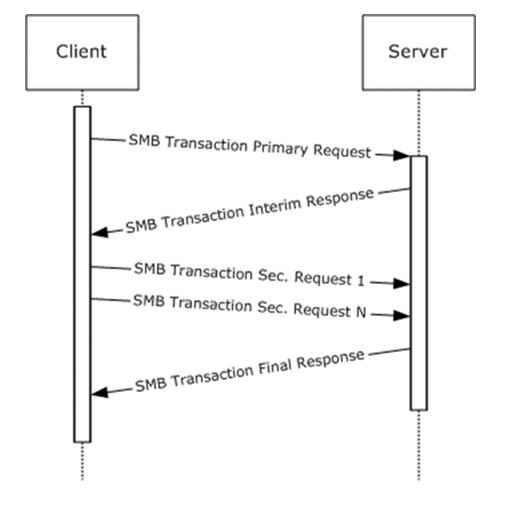
\includegraphics[width=\linewidth]{SMB-transaction.png}
	\caption{Request response, SMB protocol. Source: windows learning }
	\label{fig:SMB-transaction}
\end{figure}

\subsubsection{Buffer Overflow}
The FEAlist is a list of key/value properties which are sent with the transactions. 

\begin{itemize}
	\item The client calculates the size of the FEAlist part of the transaction and sends it to the server with the transaction.  
	\item The server allocates space in memory for the FEAlist, using pointer offsets based on the size of the list (it does not keep a 'list' variable)
	\item The size of the list is provided by the client, and checked by the server and re-calculated if the size dos not match ('All Good' right?) 
	\item However, there are multiple versions of the FEAlist format depending on the filesystem used (OS/2 vs NT). And there is a bug in the conversion of FEAlist file size between OS/2 and NT (bug in a function called "SrvOs2FeaListSizeToNt" in srv.sys \cite{h3xduck}) where only half the memory is allocated when sending a OS/2 formatted FEAlist - a 16 byte 'int' is cast to a 8 byte 'short' resulting in a buffer overflow see Ghidra analysis of code from \cite{h3xduck} in Appendix. 
\end{itemize}

\subsubsection{Secondary Transactions Race}
When the transaction size is large SMB splits it into subsequent transactions, see Figure \ref{fig:SMB-transaction}, it is \underline{the client} who tells the server where to put the subsequent packages (it provides an offset) i.e. the client (attacker) does all the bookkeeping.

\subsubsection{Heap Spraying} When sending secondary messages the input flow of data is kept open until the client sends a 'final' message i.e. the client can keep sending secondary messages directly to the heap. This enables the attacker to manipulate the memory heap with some control over where data is stored. This enables the attacker to 'groom' \cite{zerosum0x0-defcon26} the memory heap and place code for a reverse shell on the target, and eventually execute it. All data in the memory heap has execution privileges, the reverse shell has NT AUTHORITY/SYSTEM privileges - and can do anything on the client, a demo is shown in \nameref{Appendix}      


zerosum0x0-defcon26



It looks like the vulnerability was introduced as a consequence of reverse compatibility with different version of the file systems used on windows, and that a goal for file sharing with the SMB protocol is to give user experience as close to working with local files as possible.  




\section{Remediation} 
describe and explain the fix

\subsubsection{Disable buffer overflow}
Patching this was super simple (change the 8bit short to a 16bit int in the "SrvOs2FeaListSizeToNt" in srv.sys) - the problem is as always to get the patch rolled out everywhere...
The patch was actually issued before EternalBlue was published by shadowBrokers (speculation is that NSA nudged Microsoft after being aware that the leak was imminent, they had kept it secret for a long time before that, and the vulnerability showed up before)

\subsubsection{Disable "Heap Spraying"}
Newer version of Windows uses Address Space Layout Randomization (ASLR), which makes it impossible to predict and control where packages land in memory based on the offsets 




%----------------------------------------------------------------------------------------
%	 REFERENCES
%----------------------------------------------------------------------------------------

\printbibliography % Output the bibliography

%----------------------------------------------------------------------------------------
\clearpage
\appendix
\section{Appendix} \label{Appendix}

\subsection{Buffer Overflow Bug in srv.sys}
A figure from \cite{h3xduck} with code deconstructed from a vulnerable windows srv.sys is shown in \ref{fig:Ghidra_srv.sys}


\begin{figure}[ht] % Single column figure
	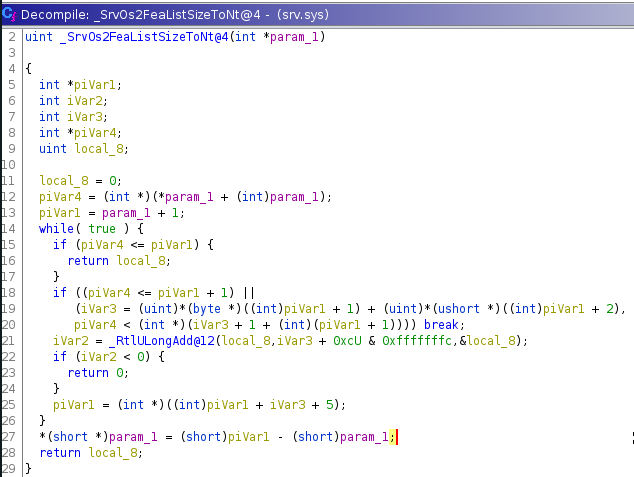
\includegraphics[width=\linewidth]{GhidraOfSrv.png}
	\caption{The buffer overflow in Srv!SrvOs2FeaToNt, deconstructed using Ghidra, figure from \cite{h3xduck}}
	\label{fig:Ghidra_srv.sys}
\end{figure}



\subsection{Metasploit}
As a demonstration of how easily the EternalBlue vulnerability can be deployed to get a system shell using Metasploit:

\subsubsection[short]{Target machine}
Early Windows 7 machine (2009), the exploit is proven to work up to 2017 where a patch was introduced (MS17-010).
Only modification is that a folder was shared on the desktop with 'user' permissions (this opens the necessary outbound rules on the firewall)

\begin{figure}[ht] % Single column figure
	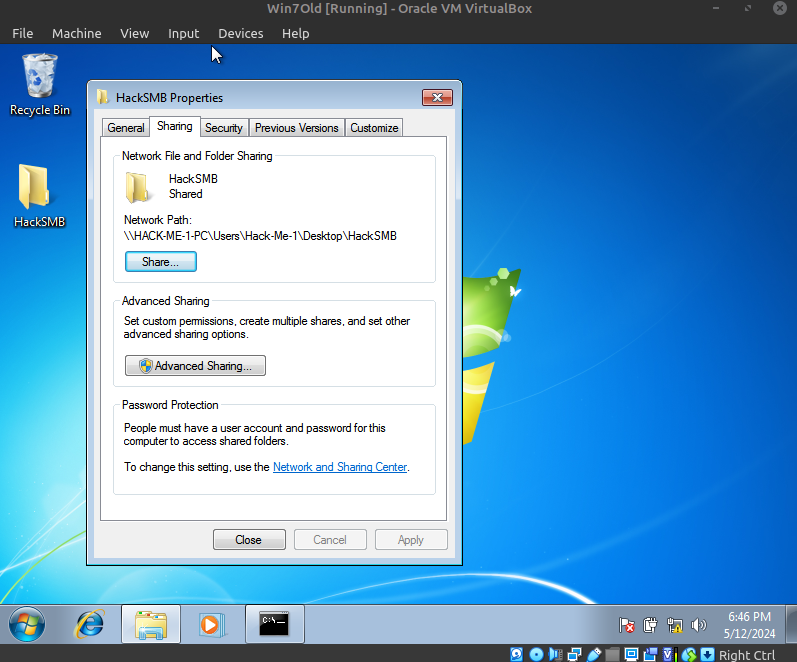
\includegraphics[width=\linewidth]{ExploitableWin7.png}
	\caption{Exploited windows 7 2009 service pack 1}
	\label{fig:ExploitableWin7}
\end{figure}

\begin{figure}[ht] % Single column figure
	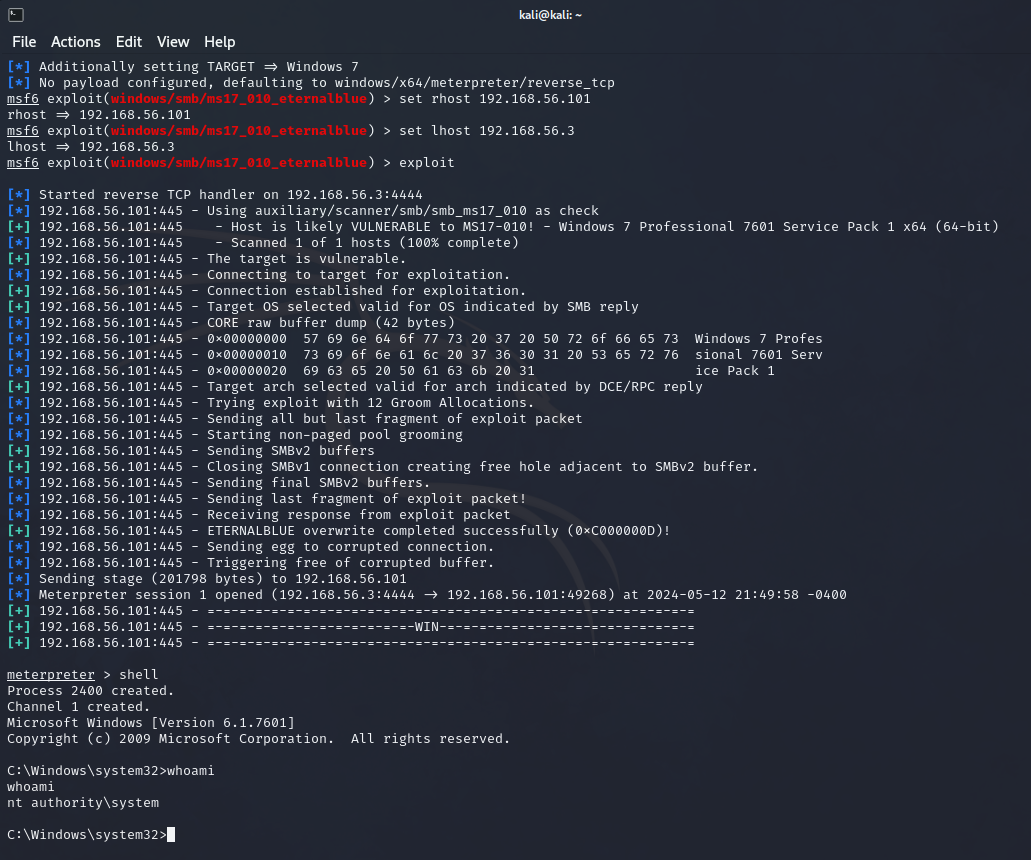
\includegraphics[width=\linewidth]{metasploit-pawned.png}
	\caption{Very easy with Metasploit}
	\label{fig:metasploit-pawned}
\end{figure}





% sudo nmap -sV 10.10.10.40  

% sudo nmap --script smb-os-discovery -p445 10.10.10.40

% sudo nmap --script smb-enum-shares -p445 10.10.10.40 


% msfconsole

% use windows/smb/ms17_010_eternalblue
% set RSHOST and LHOST

% poke around using meterpreter



% Section 5 (Optional): Appendix – include the exploit code here if you’d like to. Do NOT include the full exploit source code in Section 2


% \begin{equation}
% 	\cos^3 \theta =\frac{1}{4}\cos\theta+\frac{3}{4}\cos 3\theta
% 	\label{eq:example}
% \end{equation}

% Automatically referencing an equation number using its label: Equation \ref{eq:example}.


%------------------------------------------------








% \section{Methodologies}

% \subsection{Sample Sites \& Processing}

% This line shows how to use a footnote to further explain or cite text\footnote{Example footnote text.}.

% This is a bullet point list:

% \begin{itemize}
% 	\item Arcu eros accumsan lorem, at posuere mi diam sit amet tortor
% 	\item Fusce fermentum, mi sit amet euismod rutrum
% 	\item Sem lorem molestie diam, iaculis aliquet sapien tortor non nisi
% 	\item Pellentesque bibendum pretium aliquet
% \end{itemize}

% Mauris interdum porttitor fringilla. Proin tincidunt sodales leo at ornare. Donec tempus magna non mauris gravida luctus. Cras vitae arcu vitae mauris eleifend scelerisque. Nam sem sapien, vulputate nec felis eu, blandit convallis risus. Pellentesque sollicitudin venenatis tincidunt. In et ipsum libero. Nullam tempor ligula a massa convallis pellentesque.

% This is a numbered list:

% \begin{enumerate}
% 	\item Donec dolor arcu, rutrum id molestie in, viverra sed diam
% 	\item Curabitur feugiat
% 	\item Turpis sed auctor facilisis
% \end{enumerate}

% \subsection{Species Identification}


%------------------------------------------------

% \section{Results}

% \begin{table} % Single column table
% 	\caption{Example single column table.}
% 	\centering
% 	\begin{tabular}{l l r}
% 		\toprule
% 		\multicolumn{2}{c}{Location} \\
% 		\cmidrule(r){1-2}
% 		East Distance & West Distance & Count \\
% 		\midrule
% 		100km & 200km & 422 \\
% 		350km & 1000km & 1833 \\
% 		600km & 1200km & 890 \\
% 		\bottomrule
% 	\end{tabular}
% 	\label{tab:distcounts}
% \end{table}

% Referencing a table using its label: Table \ref{tab:distcounts}.

% \begin{table*} % Full width table (notice the starred environment)
% 	\caption{Example two column table with fixed-width columns.}
% 	\centering % Horizontally center the table
% 	\begin{tabular}{L{0.2\linewidth} L{0.2\linewidth} R{0.15\linewidth}} % Manually specify column alignments with L{}, R{} or C{} and widths as a fixed amount, usually as a proportion of \linewidth
% 		\toprule
% 		\multicolumn{2}{c}{Location} \\
% 		\cmidrule(r){1-2}
% 		East Distance & West Distance & Count \\
% 		\midrule
% 		100km & 200km & 422 \\
% 		350km & 1000km & 1833 \\
% 		600km & 1200km & 890 \\
% 		\bottomrule
% 	\end{tabular}
% \end{table*}

% \begin{figure} % Single column figure
% 	\includegraphics[width=\linewidth]{Tolmukapea.jpg}
% 	\caption{Anther of thale cress (Arabidopsis thaliana), fluorescence micrograph. Source: Heiti Paves, \href{https://commons.wikimedia.org/wiki/File:Tolmukapea.jpg}{https://commons.wiki-\\media.org/wiki/File:Tolmukapea.jpg}.}
% 	\label{fig:tcanther}
% \end{figure}

% Referencing a figure using its label: Figure \ref{fig:tcanther}.


% \begin{figure*} % Two column figure (notice the starred environment)
% 	\includegraphics[width=\linewidth]{Fibroblastid.jpg}
	% \caption{Bovine pulmonary artery endothelial cells in culture. Blue: nuclei; red: mitochondria; green: microfilaments. Computer generated image from a 3D model based on a confocal laser scanning microscopy using fluorescent marker dyes. Source: Heiti Paves, \href{https://commons.wikimedia.org/wiki/File:Fibroblastid.jpg}{https://commons.wikimedia.org/wiki/File:Fibroblastid.jpg}.}
% 	\label{fig:bpartery}
% \end{figure*}


% \subsection{Links}

% This is a clickable URL link: \href{https://www.latextemplates.com}{LaTeX Templates}. This is a clickable email link: \href{mailto:vel@latextemplates.com}{vel@latextemplates.com}. This is a clickable monospaced URL link: \url{https://www.LaTeXTemplates.com}.

%------------------------------------------------

% \section{Discussion}

% This statement requires citation \autocite{Smith:2023qr}. This statement requires multiple citations \autocite{Smith:2023qr, Smith:2024jd}. This statement contains an in-text citation, for directly referring to a citation like so: \textcite{Smith:2024jd}.

% \subsection{Subsection One}

% Suspendisse potenti. Vivamus suscipit dapibus metus. Proin auctor iaculis ex, id fermentum lectus dapibus tristique. Nullam maximus eros eget leo pretium dapibus. Nunc in auctor erat, id interdum risus. Suspendisse aliquet vehicula accumsan. In vestibulum efficitur dictum. Sed ultrices, libero nec fringilla feugiat, elit massa auctor ligula, vehicula tempor ligula felis in lectus. Suspendisse sem dui, pharetra ut sodales eu, suscipit sit amet felis. Donec pretium viverra ante, ac pulvinar eros. Suspendisse gravida consectetur urna. Pellentesque vitae leo porta, imperdiet eros eget, posuere sem. Praesent eget leo efficitur odio bibendum condimentum sit amet vel ex. Nunc maximus quam orci, quis pulvinar nibh eleifend ac. Quisque consequat lacus magna, eu posuere tellus iaculis ac. Sed vitae tortor tincidunt ante sagittis iaculis.

% \subsection{Subsection Two}

% Nullam mollis tellus lorem, sed congue ipsum euismod a. Donec pulvinar neque sed ligula ornare sodales. Nulla sagittis vel lectus nec laoreet. Nulla volutpat malesuada turpis at ultricies. Ut luctus velit odio, sagittis volutpat erat aliquet vel. Donec ac neque eget neque volutpat mollis. Vestibulum viverra ligula et sapien bibendum, vel vulputate ex euismod. Curabitur nec velit velit. Aliquam vulputate lorem elit, id tempus nisl finibus sit amet. Curabitur ex turpis, consequat at lectus id, imperdiet molestie augue. Curabitur eu eros molestie purus commodo hendrerit. Quisque auctor ipsum nec mauris malesuada, non fringilla nibh viverra. Quisque gravida, metus quis semper pulvinar, dolor nisl suscipit leo, vestibulum volutpat ante justo ultrices diam. Sed id facilisis turpis, et aliquet eros.

% \subsubsection{Subsubsection Example}

% Duis venenatis eget lectus a aliquet. Integer vulputate ante suscipit felis feugiat rutrum. Aliquam eget dolor eu augue elementum ornare. Nulla fringilla interdum volutpat. Sed tincidunt, neque quis imperdiet hendrerit, turpis sapien ornare justo, ac blandit felis sem quis diam. Proin luctus urna sit amet felis tincidunt, sed congue nunc pellentesque. Ut faucibus a magna faucibus finibus. Etiam id mi euismod, auctor nisi eget, pretium metus. Proin tincidunt interdum mi non interdum. Donec semper luctus dolor at elementum. Aenean eu congue tortor, sed hendrerit magna. Quisque a dolor ante. Mauris semper id urna id gravida. Vestibulum mi tortor, finibus eu felis in, vehicula aliquam mi.

% Aliquam arcu turpis, ultrices sed luctus ac, vehicula id metus. Morbi eu feugiat velit, et tempus augue. Proin ac mattis tortor. Donec tincidunt, ante rhoncus luctus semper, arcu lorem lobortis justo, nec convallis ante quam quis lectus. Aenean tincidunt sodales massa, et hendrerit tellus mattis ac. Sed non pretium nibh. 

% Donec cursus maximus luctus. Vivamus lobortis eros et massa porta porttitor. Nam vitae suscipit mi. Pellentesque ex tellus, iaculis vel libero at, cursus pretium sapien. Curabitur accumsan velit sit amet nulla lobortis, ut pretium ex aliquam. Proin eget volutpat orci. Morbi eu aliquet turpis. Vivamus molestie urna quis tempor tristique. Proin hendrerit sem nec tempor sollicitudin.


\end{document}
